\section{Model-based reflex agents}\label{AI: Agent Programs/Model-based reflex agents}


\begin{figure}[H]
    \centering
    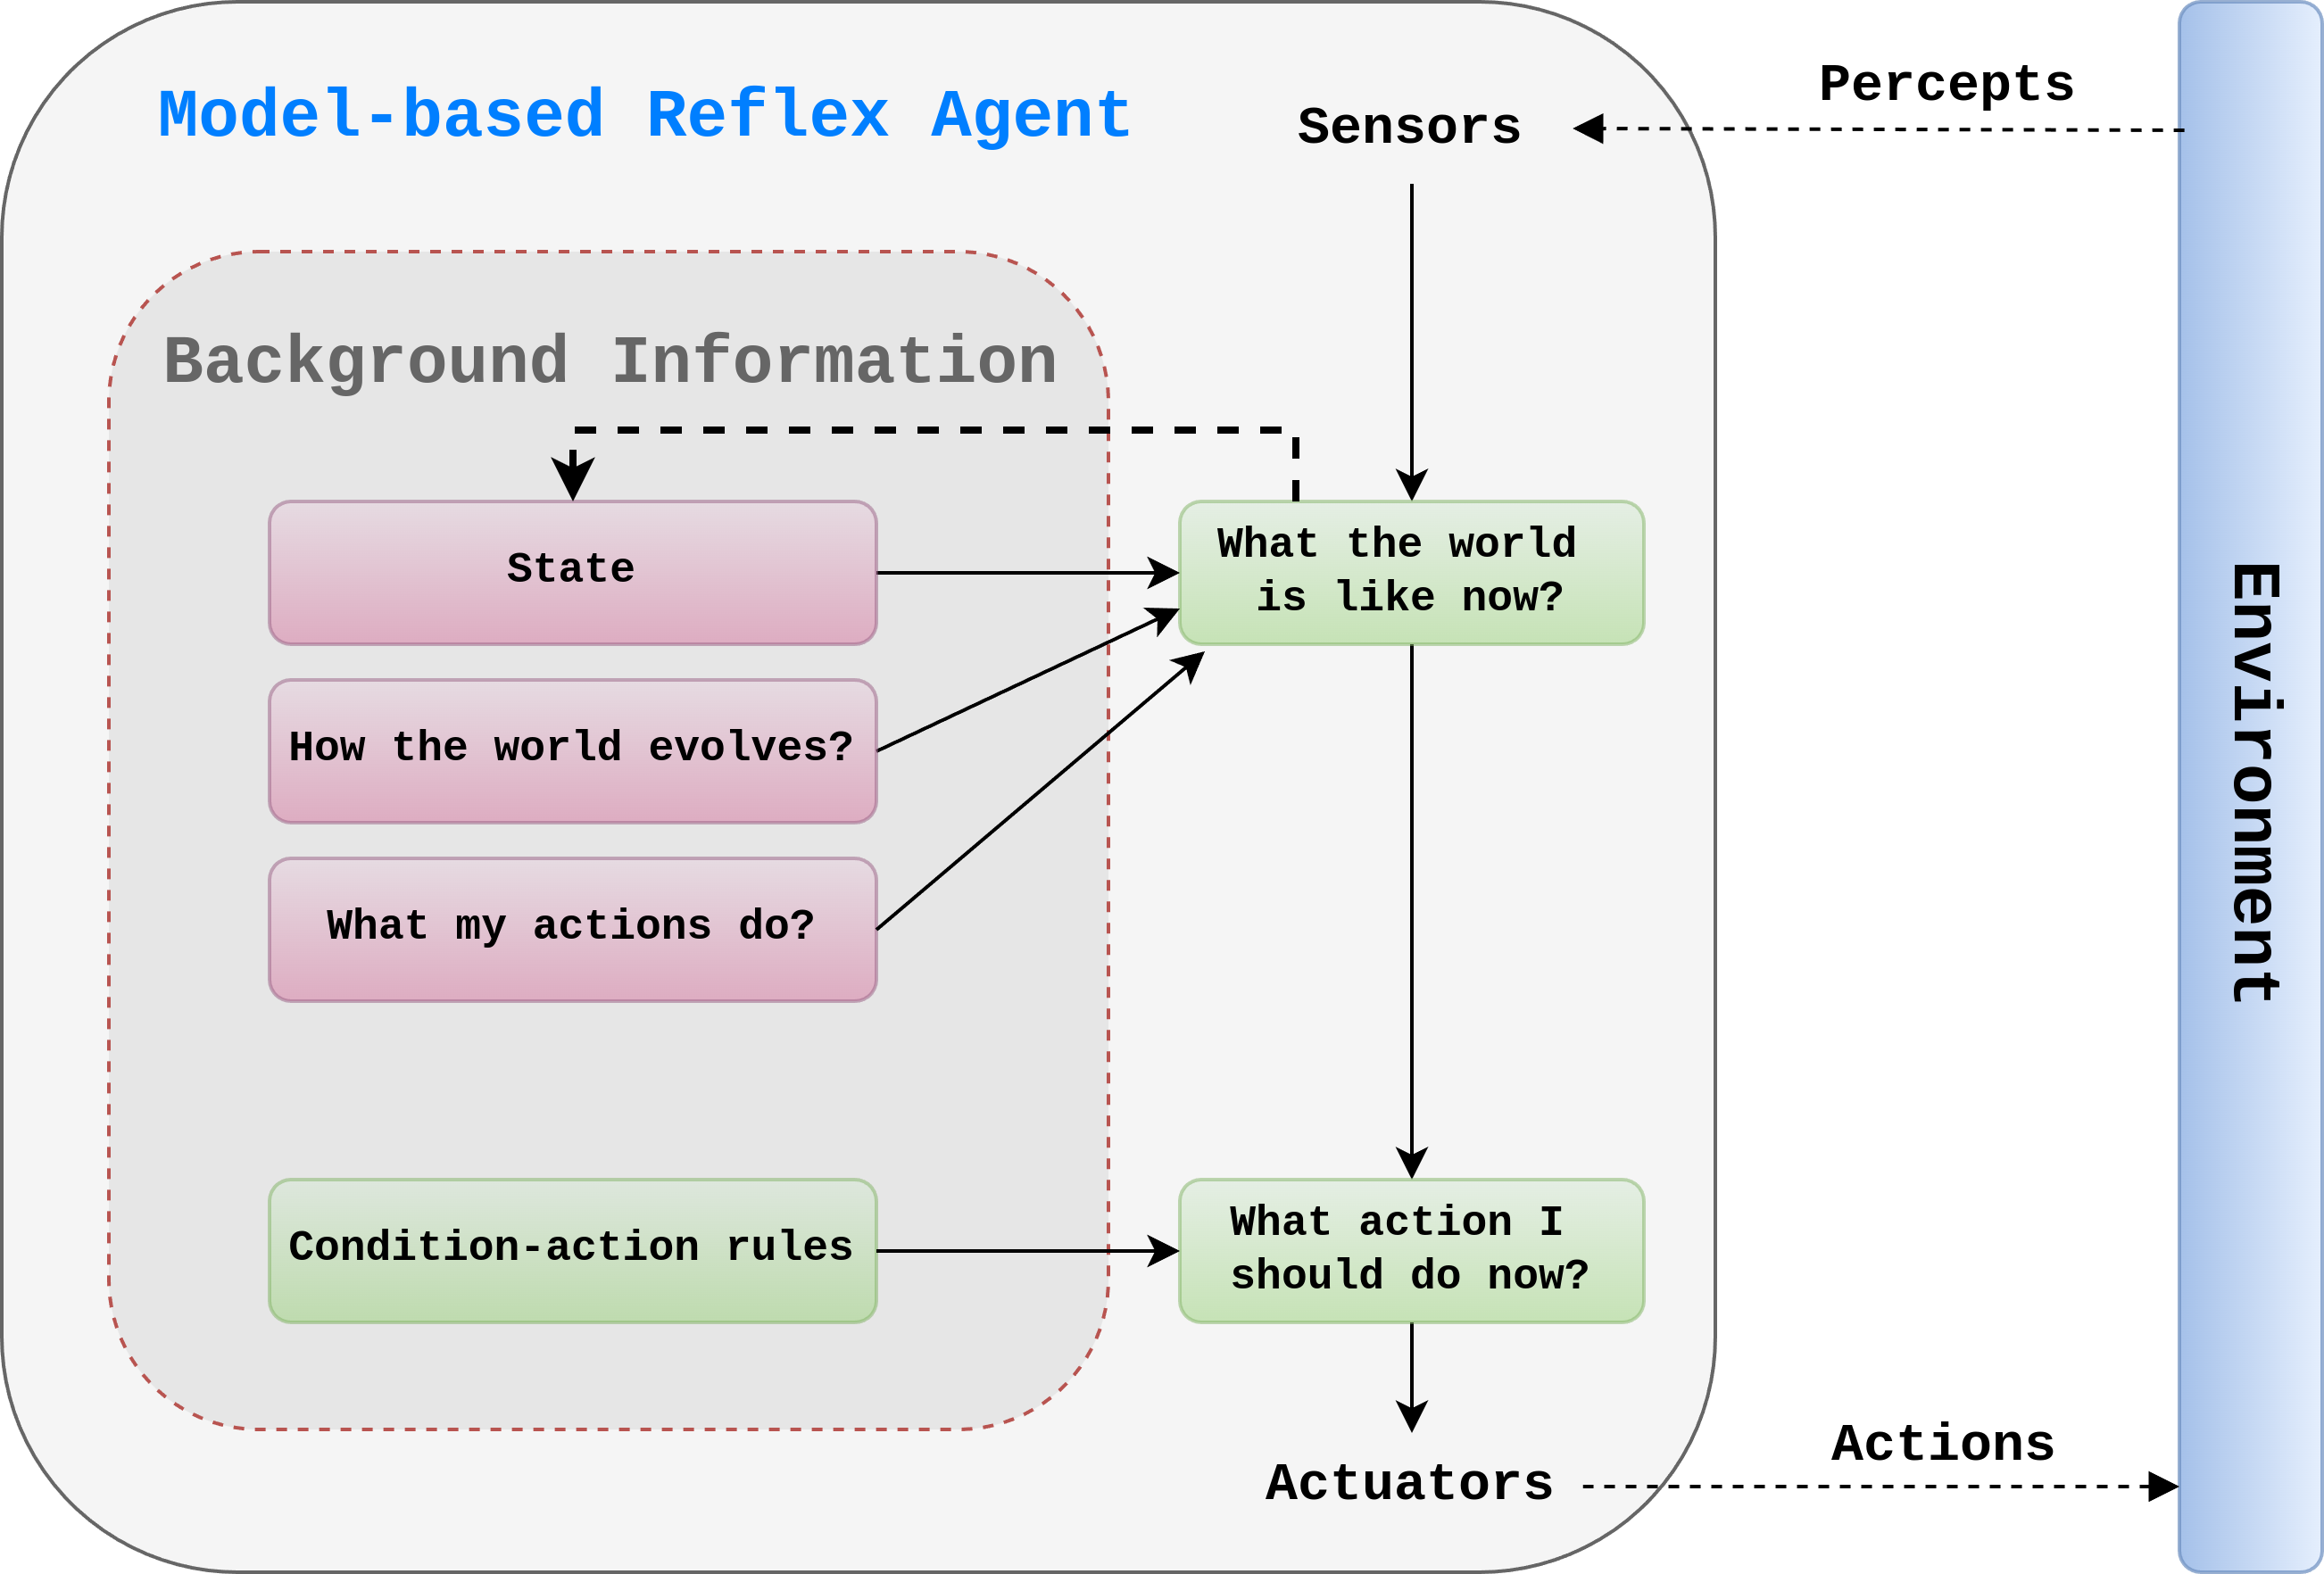
\includegraphics[
        width=0.5\linewidth, 
        height=6cm, 
        keepaspectratio
    ]{images/artificial-intelligence/ai-agents/agents-Model-based-reflex-agent.png}
    \caption*{A model-based reflex agent. \cite{common/online/tools/draw.io}}
\end{figure}


\vspace{0.2cm}

\begin{enumerate}[itemsep=0.2cm]
    \item The most effective way to handle partial observability is for the agent to keep track of the part of the world it can’t see now.
    \hfill \cite{ai/book/Artificial-Intelligence-A-Modern-Approach/Russell-Norvig}

    \item the agent should maintain some sort of internal state that depends on the percept history and thereby reflects at least some of the unobserved aspects of the current state. 
    \hfill \cite{ai/book/Artificial-Intelligence-A-Modern-Approach/Russell-Norvig}

    \item Updating this internal state information as time goes by requires two kinds of knowledge to be encoded in the agent program.
    \begin{enumerate}
        \item we need some information about how the world evolves independently of the agent
        \hfill \cite{ai/book/Artificial-Intelligence-A-Modern-Approach/Russell-Norvig}

        \item we need some information about how the agent’s own actions affect the world
        \hfill \cite{ai/book/Artificial-Intelligence-A-Modern-Approach/Russell-Norvig}
    \end{enumerate}

    \item knowledge about “how the world works” - whether implemented in simple Boolean circuits or in complete scientific theories - is called a model of the world. 
    \hfill \cite{ai/book/Artificial-Intelligence-A-Modern-Approach/Russell-Norvig}

    \item An agent that uses such a model is called a model-based agent.
    \hfill \cite{ai/book/Artificial-Intelligence-A-Modern-Approach/Russell-Norvig}

    \item Regardless of the kind of representation used, it is \textbf{seldom} possible for the agent to determine the current state of a partially observable environment \textit{exactly}.
    \hfill \cite{ai/book/Artificial-Intelligence-A-Modern-Approach/Russell-Norvig}

    \item internal “state” maintained by a model-based agent \textbf{does not} have to describe “what the world is like now” in a literal sense.
    \hfill \cite{ai/book/Artificial-Intelligence-A-Modern-Approach/Russell-Norvig}

    \item \textbf{Disadvantage}: Knowing something about the current state of the environment is \textbf{not always enough} to decide what to do.
    \hfill \cite{ai/book/Artificial-Intelligence-A-Modern-Approach/Russell-Norvig}

    \item \textbf{Disadvantage}: we would have to rewrite many condition–action rules for supporting more situations/ scenarios.     
\end{enumerate}


\vspace{0.2cm}

\begin{algorithm}[H]
    \caption{\textsc{Model-Based-Reflex-Agent}: A model-based reflex agent. It keeps track of the current state of the world, using an internal model. It then chooses an action in the same way as the reflex agent. \cite{ai/book/Artificial-Intelligence-A-Modern-Approach/Russell-Norvig}}

    \SetKwFunction{FUNCTION}{\textsc{Model-Based-Reflex-Agent}}
    \SetKwProg{Fn}{function}{ returns \normalfont an action}{end}
    \Fn{\FUNCTION{ percept }}{
        \textbf{persistent}:\\ 
            \hspace{1cm} $state$, the agent’s current conception of the world state \\
            \hspace{1cm} $model$, a description of how the next state depends on current state and action \\
            \hspace{1cm} $rules$, a set of condition-action rules \\
            \hspace{1cm} $action$, the most recent action, initially none\\
        \ \\
        $state$ $\gets$ \textsc{Update-State}( $state,\ action,\ percept,\ model$ )\\
        $rule$ $\gets$ \textsc{Rule-Match}( $state,\ rules$ ) \\
        $action$ $\gets$ $rule$.\textsc{Action} \\
        \Return $action$
    }
\end{algorithm}

\vspace{0.2cm}

\begin{enumerate}
    \item \textsc{Update-State}: responsible for creating the new internal state description. The details of how models and states are represented vary widely depending on the type of environment and the particular technology used in the agent design.
    \hfill \cite{ai/book/Artificial-Intelligence-A-Modern-Approach/Russell-Norvig}
    
\end{enumerate}













